\documentclass[11pt,letter]{article}
\usepackage{amsmath}
\usepackage{amssymb}	% packages that allow mathematical formatting
\usepackage{graphicx}	% package that allows you to include graphics
\usepackage{setspace}	% package that allows you to change spacing
\usepackage{fullpage}	% package that specifies normal margins
\usepackage{microtype}
\usepackage{amsthm}
\newcommand{\argmin}{\operatornamewithlimits{argmin}}
\renewcommand\qedsymbol{$\blacksquare$}
\usepackage{listings}
\usepackage{color}
\usepackage{subfig}


\definecolor{codegreen}{rgb}{0,0.6,0}
\definecolor{codegray}{rgb}{0.5,0.5,0.5}
\definecolor{codepurple}{rgb}{0.58,0,0.82}
\definecolor{backcolour}{rgb}{0.95,0.95,0.95}

\lstdefinestyle{mystyle}{
	backgroundcolor=\color{backcolour},   
	commentstyle=\color{codegreen},
	keywordstyle=\color{magenta},
	numberstyle=\tiny\color{codegray},
	stringstyle=\color{codepurple},
	basicstyle=\footnotesize,
	breakatwhitespace=false,         
	breaklines=true,                 
	captionpos=b,                    
	keepspaces=true,                 
	numbers=left,                    
	numbersep=5pt,                  
	showspaces=false,                
	showstringspaces=false,
	showtabs=false,                  
	tabsize=2
}

\lstset{style=mystyle}

%\usepackage[left=2.5cm, right=2.5cm, top=2cm, bottom = 3cm]{geometry}


	

\begin{document}

\begin{figure}
	\centering
	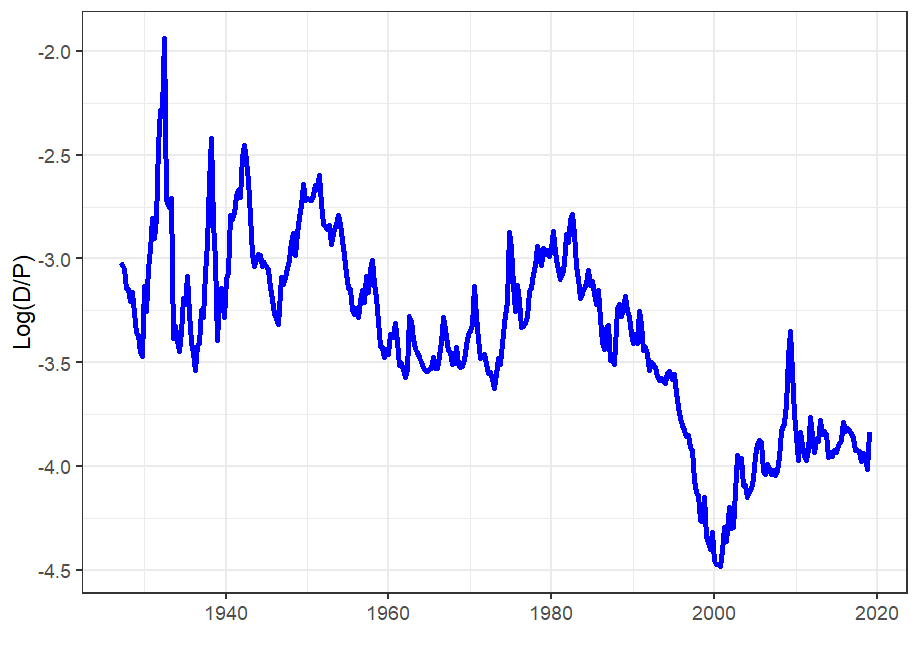
\includegraphics[scale = 0.5]{log_dividend_yield.png}
	\caption{Dividend yield (sum of past years worth of dividends divided by current portfolio price)}
	\label{fig:div_yield}
\end{figure}
\section{Problem 6}
\paragraph{a)} 
We first run two regressions separately of the form
\begin{equation*}
	\begin{split}
	r_{t, t+\tau} & = \alpha_r + \beta_{r, \tau}(d_t - p_t) + \epsilon^r_{t+\tau}\\
	\Delta d_{t, t+\tau} & = \alpha_{\Delta_d}+\beta_{\Delta d, \tau}(d_t - p_t)+ \epsilon^dp_{t+\tau}\\
	\end{split}
\end{equation*}
the results of which are shown in Table (\ref{table:div_yield_regressions}). The results suggest all variation in market price-dividend ratios corresponds to changes in expected variation in risk premiums and none about news to future dividend growth.\footnote{ Recall, we can decompose the log price dividend ratio, denoted as $z_t$ here, as
\begin{equation*}
	Var(z_t) = \sum_{j=0}^{\infty}\kappa^j_1\left[Cov(g_{t+1+j}, z_t)- Cov(r_{t+1+j}, z_t)\right]
\end{equation*}
Thus, if both returns and dividends are unforecastable, the price divdend ratio should be constant, which it clearly is not in Figure \ref{fig:div_yield}. We cannot ask "are returns forecastable?", rather we must ask "which of dividend growth or returns are forecastable?" A null hypothesis that specifies returns are not forecastable must also that dividend growth is forecastable. That is we need to test the joint distribution of return and dividend-growth forecastability. }

\begin{table}[!htbp] \centering 
	\label{} 
	\begin{tabular}{@{\extracolsep{5pt}} cccc} 
		\\[-1.8ex]\hline 
		\hline \\[-1.8ex] 
		 $\tau$ & b & t(b) & r2 \\ 
		\hline \\[-1.8ex] 
		1 & $0.078$ & $1.611$ & $0.029$ \\ 
		3 & $0.211$ & $3.050$ & $0.092$ \\ 
		5 & $0.329$ & $5.056$ & $0.173$ \\ 
		\hline \\[-1.8ex] 

	\end{tabular} 
	\quad
	\begin{tabular}{@{\extracolsep{5pt}} cccc} 
		\\[-1.8ex]\hline 
		\hline \\[-1.8ex] 
		$\tau$ & b & t(b) & r2 \\ 
		\hline \\[-1.8ex] 
	1 & $0.005$ & $0.135$ & $0.0003$ \\ 
	3 & $-0.012$ & $-0.201$ & $0.001$ \\ 
	5 & $-0.005$ & $-0.072$ & $0.0001$ \\   
		\hline \\[-1.8ex] 
	\end{tabular} 
	\caption{Direct return regressions (left panel) and dividend growth regressions (right panel)} 
	\label{table:div_yield_regressions}
\end{table} 



Next, we calculate the implied regression coefficients from our VAR and the Campbell Shiller linearization of a return
\begin{equation*}
	r_{t+1} \approx \rho + \kappa(p_{t+1} - d_{t+1}) + (d_{t+1}-d_t) - (p_t - d_t)
\end{equation*}

The implied coefficient on returns is given by
\begin{equation*}
	\beta_{r, \tau} = \frac{Cov(r_{t, t+\tau} - \tau \bar{r}, e_{1}'X_t)}{Var(e_{1}'X_t)}
\end{equation*}
We can solve for $r_{t+k} - \bar{r}$ as follows
\begin{equation}
\begin{split}
	r_{t+k} &= [-\kappa\quad 1 \quad 0] \left(X_{t+k} \right) + e_1 (X_{t+k-1}-\bar{X})\\
	&= [-\kappa\quad 1 \quad 0] \left(A(X_{t+k-1}) + \epsilon_{t+k} \right) + e_1 (X_{t+k-1})\\
	& = ([-\kappa\quad 1 \quad 0]A + e_1) X_{t+k-1} + [-\kappa\quad 1 \quad 0]\epsilon_{t+k}\\
	& = [-\kappa\quad 1 \quad 0] A^k X_t  + \sum_{j = 0}^{k-1}[-\kappa\quad 1 \quad 0] A^j\epsilon_{t+k-j} +[-\kappa\quad 1 \quad 0]\epsilon_{t+k} \\
\end{split}
\label{eq:VAR_implied_r}
\end{equation}
where the last equality holds by backwards iteration and using our VAR. Thus, $r_{t, t+\tau} - \tau \bar{r}$ is given by 
\begin{equation*}
\begin{split}
	r_{t, t+\tau}- \tau \bar{r} &= \sum_{k=1}^{\tau}(r_{t+k}-\bar{r}) \\
&= \sum_{k=1}^{\tau}\bigg([-\kappa\quad 1 \quad 0] A^k(X_t ) + \sum_{j = 0}^{k-1}[-\kappa\quad 1 \quad 0] A^j\epsilon_{t+k-j}\bigg)\\
\end{split}
\end{equation*}
 Using equation (\ref{eq:VAR_implied_r}), we can solve for our coefficient of interest. 

\begin{equation*}
	\begin{split}
     \beta_{r, \tau} &= \frac{Cov(r_{t, t+\tau} - \tau \bar{r}, e_{1}'X)}{Var(e_{1}'X)}\\
     &= \frac{Cov(\sum_{k=1}^{\tau}[-\kappa\quad 1 \quad 0] A^k(X_t ), e_{1}'X)}{Var(e_{1}'X)}\\
	\end{split}
\end{equation*}
Similarly, our coefficient for dividend growth is given by
\begin{equation*}
	\begin{split}
		\beta_{\Delta d, \tau} &= \frac{Cov(\Delta d_{t + \tau}, e_{1}'X)}{Var(e_{1}'X)}\\
		& = \frac{Cov(e_2' A^\tau X, e_{1}'X)}{Var(e_{1}'X)}\\
	\end{split}
\end{equation*}
where the equality holds, because dividend growth over $\tau$ periods implied by the VAR will just be $e_2' A^\tau X$. 
\end{document}


